%=======================================================================
%  A0 CONFERENCE POSTER
%  "Fusing Two-Stage LLM Semantic Refinement with Genetic Programming
%   for Robust Alpha Discovery and Degradation Mitigation"
%
%  Source paper : full.md / access.pdf (IEEE Access style manuscript)
%  Figures      : ./images/*.jpg  (extracted by MinerU from the PDF)
%
%  BUILD (from this folder):
%     pdflatex -interaction=nonstopmode poster.tex
%     pdflatex -interaction=nonstopmode poster.tex
%  or:  latexmk -pdf -interaction=nonstopmode poster.tex
%=======================================================================
\documentclass[final]{beamer}

% ------------------------- poster geometry ----------------------------
\usepackage[orientation=portrait, size=a0, scale=0.98]{beamerposter}

% ------------------------- fonts, maths, tools ------------------------
\usepackage[T1]{fontenc}
\usepackage[utf8]{inputenc}
\usepackage[scaled=0.92]{helvet}
\renewcommand{\familydefault}{\sfdefault}
\usepackage{lmodern}
\usepackage{amsmath,amssymb}
\usepackage{booktabs}
\usepackage{array}
\usepackage{colortbl}
\usepackage{multirow}
\usepackage{graphicx}
\usepackage{ragged2e}
\usepackage{xcolor}

% ------------------------- palette -----------------------------------
\definecolor{navy}{HTML}{0E2A47}
\definecolor{navy2}{HTML}{14456E}
\definecolor{accent}{HTML}{0091B3}
\definecolor{accent2}{HTML}{E27A1E}
\definecolor{panel}{HTML}{F2F6FA}
\definecolor{panel2}{HTML}{E4EDF6}
\definecolor{keybg}{HTML}{FFF6E8}
\definecolor{good}{HTML}{1E7B4F}
\definecolor{bad}{HTML}{B13325}
\definecolor{rule}{HTML}{C7D6E5}

% ------------------------- beamer styling -----------------------------
\setbeamercolor{block title}{fg=white, bg=navy}
\setbeamercolor{block body}{fg=black!88, bg=panel}
\setbeamerfont{block title}{size=\large, series=\bfseries}
\setbeamerfont{block body}{size=\small}
\setbeamercolor{itemize item}{fg=accent}
\setbeamercolor{itemize subitem}{fg=accent2}
\setbeamerfont{itemize/enumerate body}{size=\small}
\setbeamerfont{itemize/enumerate subbody}{size=\footnotesize}
\setbeamertemplate{itemize item}{\raisebox{0.35ex}{\small$\blacktriangleright$}}
\setbeamertemplate{itemize subitem}{\raisebox{0.35ex}{\footnotesize$\bullet$}}
\setlength{\leftmargini}{1.05cm}
\setlength{\leftmarginii}{0.9cm}
\setbeamertemplate{itemize/enumerate body begin}{\setlength{\itemsep}{0.22cm}}
\setbeamertemplate{itemize/enumerate subbody begin}{\setlength{\itemsep}{0.12cm}}

% custom block: navy headline bar + accent rule + light body panel
% NOTE: inside a beamer beamercolorbox the horizontal padding is
%       leftskip/rightskip *plus* sep on each side, while the paragraph width
%       is kept at \linewidth - 2*(leftskip+sep) *outside* the box owner's
%       control.  \linewidth therefore disagreed with the real text width and
%       every rigid item (\rule, keybox with wd=\linewidth, tables sized in
%       \linewidth, \includegraphics[width=\linewidth]) hung out of the panel.
%       We therefore set sep=0 for the body, pad with leftskip/rightskip only,
%       and re-set \linewidth to exactly the resulting text width, so rigid
%       content fits by construction.
\newlength{\blocklskip}\setlength{\blocklskip}{0.50cm}
\newlength{\blockrskip}\setlength{\blockrskip}{0.50cm}
\newlength{\blockvsep}\setlength{\blockvsep}{0.34cm}
\setbeamertemplate{block begin}{%
  \par\vskip0.50cm%
  \begin{beamercolorbox}[wd=\linewidth,leftskip=0.45cm,rightskip=0.45cm,sep=0.22cm]{block title}%
    \usebeamerfont*{block title}\insertblocktitle%
  \end{beamercolorbox}%
  \nointerlineskip%
  \hbox{\color{accent}\rule{\linewidth}{0.8ex}}%
  \nointerlineskip%
  \begin{beamercolorbox}[wd=\linewidth,vmode,leftskip=\blocklskip,rightskip=\blockrskip,sep=0cm]{block body}%
    \usebeamerfont*{block body}%
    \vskip\blockvsep%
    \setlength{\linewidth}{\dimexpr\linewidth-\blocklskip-\blockrskip\relax}%
}
\setbeamertemplate{block end}{%
  \vskip\blockvsep%
  \end{beamercolorbox}%
  \vskip0.15cm%
}
\setbeamercolor{keybox}{fg=black!85, bg=keybg}
\setbeamercolor{titlebar}{fg=white, bg=navy}
\setbeamercolor{subbar}{fg=white, bg=navy2}
\setbeamercolor{cardbox}{fg=black!85, bg=panel2}

% ------------------------- helper macros ------------------------------
% highlighted "key takeaway" box, usable inside a block
\newenvironment{keybox}[1]{%
  \par\vskip0.32cm\noindent%
  \begin{beamercolorbox}[wd=\linewidth,leftskip=0.35cm,rightskip=0.35cm,sep=0.3cm]{keybox}%
  \textbf{\color{accent2}#1}\par\vskip0.12cm%
}{%
  \end{beamercolorbox}\vskip0.22cm\par%
}
\newcommand{\hl}[1]{\textbf{\color{navy2}#1}}
\newcommand{\gd}[1]{\textbf{\color{good}#1}}
\newcommand{\bd}[1]{\textbf{\color{bad}#1}}
\newcommand{\code}[1]{\texttt{#1}}
\newcommand{\figcap}[1]{\par\vskip0.25cm{\small\itshape #1}\par}
% metric card for the header strip
\newcommand{\metriccard}[2]{%
  \begin{minipage}[t]{\linewidth}\centering
    {\fontsize{30}{36}\selectfont\bfseries\color{navy2}#1}\par\vskip0.16cm
    {\small #2}
  \end{minipage}%
}
\newcolumntype{L}[1]{>{\raggedright\arraybackslash}p{#1}}
\newcolumntype{C}[1]{>{\centering\arraybackslash}p{#1}}
\setlength{\overfullrule}{4pt}% TODO: remove before final build (debug aid)

\begin{document}
\begin{frame}[t]{}

%================== TITLE BAR =========================================
\begin{beamercolorbox}[wd=\textwidth,leftskip=0.8cm,rightskip=0.8cm,sep=0.5cm,center]{titlebar}
  {\normalsize\bfseries\color{accent!45!white}
   IEEE ACCESS \textbullet\ QUANTITATIVE FINANCE \textbullet\ NEURO-SYMBOLIC ALPHA DISCOVERY}\par\vskip0.35cm
  {\fontsize{46}{54}\selectfont\bfseries
   Fusing Two-Stage LLM Semantic Refinement with Genetic Programming\\[0.1cm]
   for Robust Alpha Discovery and Degradation Mitigation}\par\vskip0.32cm
  {\large G.\,S.\,K. Raghav Anand$^{1}$, Second Author$^{2}$, Third Author$^{3}$}\par\vskip0.15cm
  {\small $^{1}$Dept.\ of Computer Science \& Engineering, National Institute of Technology, India
   \ \textbullet\ \ $^{2}$Dept.\ of Quantitative Finance, Financial Engineering Laboratory, India
   \ \textbullet\ \ $^{3}$School of Artificial Intelligence, Advanced Computing Institute, India}\par\vskip0.18cm
  {\small Contact: \code{author@institution.edu} \ \textbullet\ Supported in part by the Advanced Quantitative Research Initiative (Project CAP-2026)}
\end{beamercolorbox}

%================== IMPACT STRIP ======================================
\begin{beamercolorbox}[wd=\textwidth,leftskip=0.8cm,rightskip=0.8cm,sep=0.4cm]{cardbox}
\begin{columns}[t]
  \begin{column}{0.197\textwidth}\metriccard{0.5518$\rightarrow$0.6365}{Net Sharpe, Nifty 50 (+15.3\% relative; peak 0.6465)}\end{column}
  \begin{column}{0.197\textwidth}\metriccard{9.61\% / 10.63\%}{Annualised net return, deterministic / peak (ceiling 8.41\%)}\end{column}
  \begin{column}{0.197\textwidth}\metriccard{$-$35\%$\rightarrow-$6.8\%}{OOS Sharpe decay, US S\&P 500 (Vanilla GP $\rightarrow$ ours)}\end{column}
  \begin{column}{0.197\textwidth}\metriccard{$-$92\%$\rightarrow-$46.7\%}{OOS Sharpe decay halved on China SSE Composite}\end{column}
  \begin{column}{0.197\textwidth}\metriccard{38.8 min \textbullet\ \$0}{Full local run, 8-bit quantised LLMs, no API cost, $T{=}0.0$}\end{column}
\end{columns}
\end{beamercolorbox}

\vskip0.45cm
\begin{columns}[t]
%======================================================================
%  COLUMN 1
%======================================================================
\begin{column}{0.325\textwidth}

\begin{block}{1 \; Why GP Alphas Break: Semantic Overfitting}
\begin{itemize}
  \item \hl{Genetic Programming (GP)} discovers auditable formulaic alphas by searching trees of financial operators --- yet it optimises \emph{only} statistical fitness (Rank-IC / ICIR) on historical data.
  \item GP therefore cannot separate economically grounded relationships from spurious mathematical artifacts, and selects formulas that fit \emph{structural noise}.
  \item Hall-of-Fame pathologies observed in our runs: \code{cos(close)}, \code{sin(price\_to\_sma20)}, \code{sub(close, volume)} (a currency price minus a share count), \code{mul(cos(pe\_ratio), ret\_5d)}: brilliant in-sample, \bd{decaying $-35.03\%$ (US) and $-92.08\%$ (China)} out-of-sample.
  \item Prior LLM remedies are \emph{destructive}: TEDE prunes subtrees syntactically, AlphaAgent rejects candidates terminally. Because \hl{$>80\%$} of evolved expressions carry minor dimensional or syntactic imperfections, rejection causes devastating formula attrition and wastes hard-won predictive structure.
\end{itemize}
\begin{keybox}{Core idea --- reject $\neq$ repair}
Instead of discarding a flawed candidate, the refiner \textbf{repairs} the flawed sub-expression under a \emph{closed financial grammar} and compiles it back into the evaluation loop, preserving the valid predictive structure that evolution already discovered.
\end{keybox}
\end{block}

\begin{block}{2 \; Contributions}
\begin{enumerate}
  \item \hl{Dual two-stage framework}: a regime-aware GP ensemble (AFM macro fusion + HMM market states) coupled with a conditional Two-Stage LLM Semantic Refiner in which a semantic failure ($S \leq 2$) triggers domain-constrained repair rather than rejection.
  \item \hl{Closed-vocabulary hallucination control}: a strict feature ($\mathcal{F}$) / operator ($\mathcal{O}$) grammar guarantees that \gd{100\%} of LLM-repaired formulas compile into valid Abstract Syntax Trees, with zero runtime variable hallucination.
  \item \hl{Empirical alpha discovery}: 9.61\% deterministic / 10.63\% peak annualised net return and net Sharpe 0.6365--0.6465 on a 23-year Nifty 50 panel, beating momentum, low-volatility, mean reversion, Vanilla GP and the pre-LLM regime ensemble.
  \item \hl{Cross-market degradation mitigation}: OOS Sharpe decay on the S\&P 500 is compressed from $-35.03\%$ to $-6.77\%$ and halved on the SSE --- evidence that closed-vocabulary semantic repair acts as a structural regulariser against historical noise overfitting.
\end{enumerate}
\end{block}

\begin{block}{3 \; Data, Protocol \& Evaluation}
\begin{itemize}
  \item \hl{Panel}: NSE Nifty 50 constituents ($N = 50$), $T = 5{,}834$ daily bars (2002--2025), feature vector $\mathbf{x}_{i,t} \in \mathbb{R}^{28}$ --- price/volume, momentum (5/20/60 d), volatility scalers, drawdowns, RSI, Bollinger bands, valuation ratios, FinBERT news sentiment and macro trend.
  \item \hl{Objective}: forward 20-day cross-sectional return (Eq.~1); alphas rank stocks cross-sectionally (Eq.~2) and are scored by Spearman Rank IC (Eq.~3) and ICIR (Eq.~4).
  \item \hl{Strict temporal split}: GP evolution + HMM training 2002--2015 \textbullet\ validation 2016--2018 \textbullet\ out-of-sample test 2019--2025 (1,729 trading days). Annual fundamentals stay fiscal-year aligned and forward-filled to prevent look-ahead leakage.
  \item \hl{Portfolio}: dollar-neutral top/bottom quintile, 20-day holding horizon, 10 bps round-trip friction. Reported metrics: annualised net return, net Sharpe, Rank IC, ICIR, maximum drawdown, win rate and turnover.
\end{itemize}
\vskip0.15cm
\begin{align*}
r_{i,t+h} &= \frac{P_{i,t+h}-P_{i,t}}{P_{i,t}}\,,\quad h=20\ \text{d} \qquad \text{(1)}\\[0.15cm]
\mathrm{RankIC}_t &= \rho_{\text{Spearman}}\big(\alpha(\mathbf{x}_{i,t}),\, r_{i,t+h}\big) \qquad \text{(3)}\\[0.15cm]
\mathrm{ICIR} &= \frac{\overline{\mathrm{RankIC}}}{\sigma_{\mathrm{RankIC}}+\epsilon}\,,\qquad \epsilon = 10^{-8} \qquad \text{(4)}
\end{align*}
\end{block}

\begin{block}{4 \; Theory: Compressing the Hypothesis Space}
\begin{itemize}
  \item \hl{Combinatorial explosion}: with $|\mathcal{O}| = 13$ operators and $|\mathcal{F}| = 28$ terminals, the unrestricted syntactic space at depth $D$ contains
  $|\mathcal{H}_{\mathrm{raw}}(D)| = |\mathcal{O}|^{2^{D}-1}\cdot|\mathcal{F}|^{2^{D}}$
  (Eq.~5) --- already $\approx 2.4\times 10^{39}$ distinct trees at depth $D = 4$.
  \item \hl{Generalisation bound} (Eq.~6): the out-of-sample gap scales with the empirical Rademacher complexity $\mathcal{R}_n(\mathcal{H})$, which follows the pseudo-dimension of the hypothesis class. For $\mathcal{H}_{\mathrm{raw}}$ that dimension is enormous, explaining the severe decay of standard GP.
  \item \hl{Economic projection} (Eq.~7): the closed vocabulary together with the LLM refiner implements
  $\Pi_{\mathrm{econ}}:\mathcal{H}_{\mathrm{raw}} \to \mathcal{H}_{\mathrm{sound}}$, eliminating dimensionally absurd operators, periodic functions on price levels and spurious high-frequency noise, so that
  $\mathcal{R}_n(\mathcal{H}_{\mathrm{sound}}) \ll \mathcal{R}_n(\mathcal{H}_{\mathrm{raw}})$.
\end{itemize}
\vskip0.1cm
\[
\sup_{f\in\mathcal{H}}\bigl|\mathcal{L}_{\mathrm{OOS}}(f)-\mathcal{L}_{\mathrm{IS}}(f)\bigr| \;\leq\; 2\,\mathcal{R}_n(\mathcal{H}) \;+\; \mathcal{O}\!\left(\sqrt{\frac{\ln(1/\delta)}{n}}\,\right) \qquad \text{(6)}
\]
\end{block}

\begin{block}{5 \; Cross-Market Degradation Mitigation}
{\small
\setlength{\tabcolsep}{0.22cm}
\renewcommand{\arraystretch}{1.32}
\begin{tabular}{@{}L{0.28\linewidth}L{0.26\linewidth}C{0.13\linewidth}L{0.21\linewidth}@{}}
\toprule
\textbf{Market} & \textbf{Architecture} & \textbf{IS Sharpe} & \textbf{OOS Sharpe (decay)}\\
\midrule
\multirow{3}{*}{US S\&P 500} & Vanilla GP & 1.393 & 0.905 (\bd{$-35.03\%$})\\
 & HMM Regime-GP & 1.228 & 0.974 (\bd{$-20.71\%$})\\
 & \hl{Proposed framework} & 1.153 & \gd{1.075 ($-6.77\%$)}\\
\midrule
\multirow{3}{*}{China SSE} & Vanilla GP & 0.436 & 0.035 (\bd{$-92.08\%$})\\
 & HMM Regime-GP & 0.633 & 0.232 (\bd{$-63.28\%$})\\
 & \hl{Proposed framework} & 0.126 & \gd{0.067 ($-46.68\%$)}\\
\midrule
\multirow{3}{*}{India Nifty 50} & Vanilla GP & 0.954 & 0.5518 (\bd{$-42.16\%$})\\
 & HMM Regime-GP & 0.814 & 0.5244 (\bd{$-35.62\%$})\\
 & \hl{Proposed framework} & 0.957 & \gd{0.6365 ($-33.49\%$)}\\
\bottomrule
\end{tabular}}
\begin{keybox}{Degradation is the real target}
On the efficient S\&P 500 the framework attains the \gd{highest OOS Sharpe (1.075)} from the \gd{lowest} in-sample Sharpe --- decay cut \gd{5$\times$} (US) and \gd{$\sim$2$\times$} (China SSE).
\end{keybox}
\end{block}

\begin{block}{6 \; Friction Sensitivity of Net Alpha (Table 7)}
{\footnotesize
\setlength{\tabcolsep}{0.24cm}
\renewcommand{\arraystretch}{1.22}
\begin{tabular}{@{}L{0.30\linewidth}C{0.17\linewidth}C{0.17\linewidth}C{0.17\linewidth}@{}}
\toprule
\textbf{Round-trip friction} & \textbf{Ann. return} & \textbf{Net Sharpe} & \textbf{Max DD}\\
\midrule
0 bps (frictionless) & 11.84\% & 0.7420 & $-18.21\%$\\
\rowcolor{panel2}
\textbf{10 bps (baseline)} & \gd{9.61\%} & \gd{0.6365} & $-19.68\%$\\
20 bps & 7.38\% & 0.5098 & $-21.16\%$\\
30 bps (stress test) & 5.15\% & 0.3831 & $-22.65\%$\\
\bottomrule
\end{tabular}}
\vskip0.12cm
Each extra 5 bps of friction costs $\sim$1.11\% p.a.\ (20-day rebalancing, $\sim$14.8\% turnover); the \gd{38.4 bps break-even} far exceeds the 4--8 bps cost of liquid NIFTY 50 execution, so the alpha is not a churning artifact.
\end{block}

\end{column}
%======================================================================
%  COLUMN 2
%======================================================================
\begin{column}{0.325\textwidth}

\begin{block}{7 \; System Architecture}
\centering
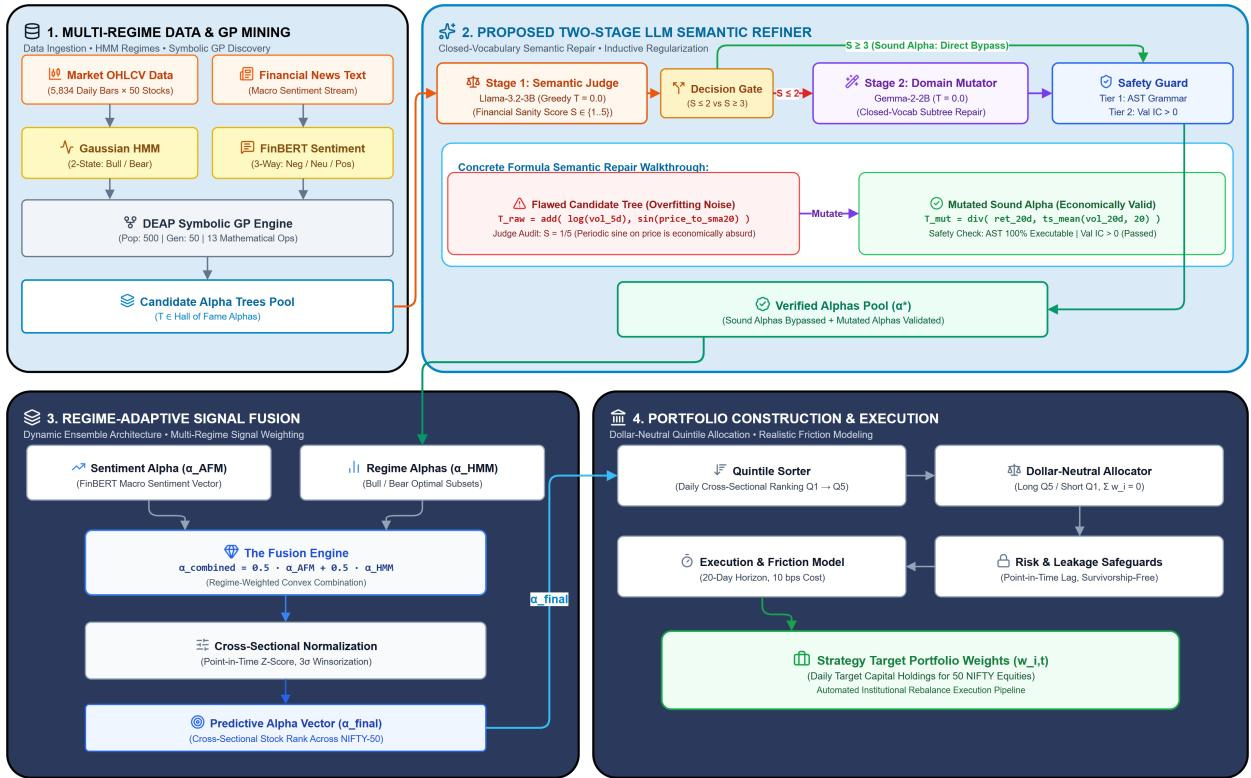
\includegraphics[width=0.95\linewidth]{images/38de923ab8b5dcfc8845af49392f1122074f030c0adba45a84530c30bf42c1bf.jpg}
\figcap{Figure 1. Dual two-stage framework: (1) the regime-aware factor engine (AFM macro regimes $+$ HMM states $+$ regime-specialised GP evolution) and (2) the post-evolution Two-Stage LLM Semantic Refiner (Llama-3B judge, Gemma-2B closed-vocabulary repair at $T{=}0.0$) with AST and validation guards.}
\end{block}

\begin{block}{8 \; Stage 1 --- Regime-Aware Factor Engine}
\begin{itemize}
  \item \hl{AFM macro anchor (FinALFA)}: $\sim$300k news articles are entity-matched and business-keyword filtered; FinBERT sentiment is fused with sector-standardised fundamental ratios through a learned scalar $\alpha^{*}\in[0,1]$:
  \[ x_t(\alpha) = \alpha^{*}\tilde{S}_t + (1-\alpha^{*})\tilde{F}_t \qquad \text{(8)} \]
  \item \hl{Gaussian HMM}: a two-state HMM (Baum--Welch, NIFTY-50 index) yields a persistent expansion state (State 0: 72.5\% occupancy, $P(0{\to}0)=0.994$) and a turbulence state (State 1: 27.5\%, $P(1{\to}1)=0.983$), giving each GP engine a consistent, regime-delineated training slice.
  \item \hl{Regime-specialised GP}: two DEAP populations evolve in parallel, each conditioned on its own latent state, with validation ICIR as fitness (population 500, 50 generations, depth $\leq 6$, tournament 7, $P_c=0.7$, $P_m=0.1$, parsimony $\lambda=0.002$):
  \[ \mathcal{P}_{\mathrm{Bull}} \sim \mathrm{Fitness}(\alpha \mid \hat{s}_t = 0), \quad \mathcal{P}_{\mathrm{Bear}} \sim \mathrm{Fitness}(\alpha \mid \hat{s}_t = 1) \qquad \text{(9)} \]
  \item \hl{Economic specialisation}: bull engines select momentum and volatility-scaled terms riding institutional flows; bear engines shift to mean reversion, drawdown and valuation metrics capturing liquidity overreaction.
\end{itemize}
\end{block}

\begin{block}{9 \; Stage 2 --- Two-Stage LLM Refiner}
\noindent\begin{minipage}[t]{0.475\linewidth}
\textbf{\color{accent2}Stage 1 --- economic judge (Llama-3.2-3B-Instruct)}\\[0.12cm]
Each Hall-of-Fame tree is scored on a \hl{5-point financial sanity rubric} under greedy decoding ($T = 0.0$).\\[0.1cm]
\textbf{Decision gate:} $S \geq 3$ $\Rightarrow$ \gd{direct bypass}; only $S \leq 2$ is escalated to repair. Neutral formulas ($S{=}3$) often encode genuine nonlinear structure that heuristics misread --- rewriting them destroyed performance.
\end{minipage}\hfill
\begin{minipage}[t]{0.495\linewidth}
\textbf{\color{accent2}Stage 2 --- domain-constrained mutator (Gemma-2-2B-IT)}\\[0.12cm]
Repair is deterministic ($T = 0.0$) and confined \emph{to the closed vocabulary}:
{\footnotesize\[\mathcal{T}_{\text{mut}} \sim \mathrm{LLM}_{\text{Gemma}}\bigl(\mathrm{Prompt}(\mathcal{T}_{\text{failed}},\mathcal{F},\mathcal{O})\bigr) \quad \text{(10)}\]}
\textbf{Two-tier guard:} Tier 1 parses the rewrite against $\mathcal{G}(\mathcal{F},\mathcal{O})$ and checks for variable hallucination; Tier 2 requires $IC_{\text{val}}(\mathcal{T}_{\text{mut}}) > 0$; otherwise the pipeline \emph{safely falls back} to the original candidate.
\end{minipage}
\vskip0.18cm
\textbf{Final ensemble blend} (point-in-time z-score normalisation):
\[ \alpha_{\text{final}} = \mathrm{zscore}\bigl(0.5\cdot\alpha_{\text{Ensemble,LLM}} \;+\; 0.5\cdot\alpha_{\text{HMM,LLM}}\bigr) \qquad \text{(11)} \]
\end{block}

\begin{block}{10 \; Closed Vocabulary: Zero-Hallucination Grammar (Table 2)}
{\footnotesize
\setlength{\tabcolsep}{0.22cm}
\renewcommand{\arraystretch}{1.25}
\begin{tabular}{@{}L{0.19\linewidth}L{0.75\linewidth}@{}}
\toprule
\textbf{Features} $\mathcal{F}$ \textbf{(28)} & \code{open}, \code{high}, \code{low}, \code{close}, \code{volume}, \code{ret\_5d}, \code{ret\_20d}, \code{ret\_60d}, \code{vol\_5d}, \code{vol\_20d}, \code{vol\_60d}, \code{dd\_20d}, \code{dd\_60d}, \code{price\_to\_sma20}, \code{price\_to\_sma50}, \code{rsi\_14}, \code{bb\_upper}, \code{bb\_lower}, \code{pe\_ratio}, \code{pb\_ratio}, \code{roe}, \code{roce}, \code{debt\_to\_equity}, \code{current\_ratio}, \code{sentiment\_score}, \code{afm\_fundamental}, \code{afm\_sentiment}, \code{macro\_trend}\\
\midrule
\textbf{Operators} $\mathcal{O}$ \textbf{(13)} & \code{add(a,b)}, \code{sub(a,b)}, \code{mul(a,b)}, \code{div(a,b)}, \code{neg(a)}, \code{abs(a)}, \code{log(a)}, \code{inv(a)}, \code{ts\_mean(a,d)}, \code{ts\_max(a,d)}, \code{ts\_min(a,d)}, \code{rank(a)}\\
\bottomrule
\end{tabular}}
\vskip0.1cm
\gd{100\%} of repaired expressions compiled to valid ASTs and executed without a single runtime exception across all 1,729 out-of-sample days.
\end{block}

\begin{block}{11 \; Semantic Repair in Action: Three Audited Cases}
\begin{itemize}
  \item \hl{Periodic artifact removal.} Flawed ($S{=}1/5$): \code{add(log(vol\_5d), sin(price\_to\_sma20))}. \emph{Judge:} a sine cannot model price cyclicality --- it injects spurious in-sample noise. Repaired ($S{=}4/5$): \code{div(ret\_20d, ts\_mean(vol\_20d,20))}, risk-adjusted momentum; Rank IC $-0.012 \to +0.038$.
  \item \hl{Dimensional repair.} Flawed ($S{=}1/5$): \code{sub(close, volume)} --- a currency price minus a share count. \emph{Judge:} dimensional violation, no economic meaning. Repaired ($S{=}5/5$): \code{(close - ts\_mean(close,20))/ts\_std(close,20)}, a standardised price z-score.
  \item \hl{Overfitting-noise smoothing.} Flawed ($S{=}2/5$): \code{mul(cos(pe\_ratio), ret\_5d)}. \emph{Judge:} cosine modulation of P/E multiples overfits sample noise. Repaired ($S{=}4/5$): \code{div(pe\_ratio, ts\_mean(pe\_ratio,60))} --- a relative-valuation discount metric.
\end{itemize}
\end{block}

\begin{block}{12 \; Compute \& Token Economics (Table 8)}
\begin{itemize}
  \item \hl{Where the time goes}: parallel GP evolution dominates at \bd{38.5 min} (0.82 ms/individual); AFM 7.0 s, HMM fit 4.5 s, AST guard 0.02 s --- \gd{38.8 min} end-to-end on one local workstation.
  \item \hl{Refinement is almost free}: only the 50 Hall-of-Fame candidates are refined, so Stage 1 (138 ms/expr, 6.9 s) and Stage 2 (295 ms/expr, 7.4 s) together cost under 15 s; 8-bit weights peak at 4.2 / 3.8 GB VRAM, zero API spend.
\end{itemize}
\end{block}

\begin{block}{13 \; Reproducible Protocol: Algorithm 1 (Table 3)}
{\footnotesize
\setlength{\tabcolsep}{0.26cm}
\renewcommand{\arraystretch}{1.04}
\begin{tabular}{@{}r@{\hskip0.3cm}L{0.80\linewidth}@{}}
1 & $A^{*} \leftarrow \emptyset$ \hfill \emph{(verified alpha pool)}\\
2 & \textbf{for each} Hall-of-Fame candidate $T \in \mathcal{T}_{\text{raw}}$ \textbf{do}\\
3 & \quad $S \leftarrow \mathrm{LLM}_{\text{Judge}}(T) \in \{1,\dots,5\}$ \hfill \emph{Stage 1: Llama-3.2-3B, $T{=}0.0$}\\
4 & \quad \textbf{if} $S \leq \tau = 2$ \textbf{then} $\mathcal{T}_{\text{flawed}} \leftarrow$ flawed sub-expression of $T$;\\
  & \quad\quad $\mathcal{T}_{\text{mut}} \leftarrow \mathrm{LLM}_{\text{Mutator}}(\mathcal{T}_{\text{flawed}}, \mathcal{F}, \mathcal{O})$ \hfill \emph{Stage 2: Gemma-2-2B, $T{=}0.0$}\\
5 & \quad\quad \textbf{if} AST-ok$(\mathcal{T}_{\text{mut}},\mathcal{G}(\mathcal{F},\mathcal{O}))$ \textbf{and} $IC_{\text{val}}(\mathcal{T}_{\text{mut}}) > 0$ \textbf{then} $A^{*} \leftarrow A^{*} \cup \{\mathcal{T}_{\text{mut}}\}$\\
  & \quad\quad \textbf{else} $A^{*} \leftarrow A^{*} \cup \{T\}$ \hfill \emph{safe fallback}\\
6 & \quad \textbf{else} $A^{*} \leftarrow A^{*} \cup \{T\}$ \hfill \emph{$S \geq 3$: direct bypass (sound alpha)}\\
7 & \textbf{return} $A^{*}$ \hfill \emph{verified, economically sound alpha set}\\
\end{tabular}}
\end{block}

\end{column}
\begin{column}{0.325\textwidth}

\begin{block}{14 \; Main Out-of-Sample Results (Table 4)}
{\footnotesize
\setlength{\tabcolsep}{0.24cm}
\renewcommand{\arraystretch}{1.24}
\begin{tabular}{@{}L{0.40\linewidth}C{0.14\linewidth}C{0.16\linewidth}C{0.14\linewidth}@{}}
\toprule
\textbf{Strategy} & \textbf{Ann. net return} & \textbf{Net Sharpe} & \textbf{Max DD}\\
\midrule
Momentum (12-1M) & $-2.57\%$ & $-0.1369$ & $-40.65\%$\\
Low volatility & $-10.24\%$ & $-0.5454$ & $-65.71\%$\\
Mean reversion & 4.46\% & 0.2981 & $-20.19\%$\\
Vanilla GP & 1.62\% & 0.4417 & $-4.82\%$\\
AFM adaptive fusion & 4.08\% & 0.2785 & $-19.34\%$\\
HMM regime-GP alpha & 7.49\% & 0.5244 & $-18.17\%$\\
Regime-GP ensemble + HMM (pre-LLM) & 8.41\% & 0.5518 & $-19.62\%$\\
\midrule
\rowcolor{panel2}
\textbf{Proposed: Llama-3B + Gemma-2B (det.)} & \gd{9.61\%} & \gd{0.6365} & $-19.59\%$\\
\rowcolor{panel2}
\textbf{Proposed: Llama-3.2-3B (peak)} & \gd{10.63\%} & \gd{0.6465} & $-19.59\%$\\
\bottomrule
\end{tabular}}
\vskip0.15cm
Both proposed rows lift the \hl{quantitative ceiling} (8.41\% / 0.5518) without inflating drawdown, raising the win rate to \gd{60.4\%} and ICIR to \gd{0.1650} (0.1381 pre-LLM). DeepSeek-1.5B and Gemma-2B judges left returns at 8.41\% and Qwen-2.5-3B reached 8.60\%.
\end{block}

\begin{block}{15 \; Ablation Ladder \& Hyperparameters (Table 5)}
{\footnotesize
\setlength{\tabcolsep}{0.24cm}
\renewcommand{\arraystretch}{1.24}
\begin{tabular}{@{}L{0.38\linewidth}C{0.14\linewidth}C{0.13\linewidth}C{0.13\linewidth}C{0.12\linewidth}@{}}
\toprule
\textbf{Configuration} & \textbf{Ann. return} & \textbf{Sharpe} & \textbf{Rank IC} & \textbf{Max DD}\\
\midrule
Vanilla GP & 1.62\% & 0.44 & 0.0130 & $-4.82\%$\\
GP (AFM-Bear only) & 6.43\% & 0.48 & 0.0358 & $-23.42\%$\\
HMM regime-GP alpha & 7.49\% & 0.52 & 0.0303 & $-18.17\%$\\
Regime-GP soft/hard blend & 7.52\% & 0.56 & 0.0381 & $-23.42\%$\\
Regime-GP ensemble (pre-LLM) & 8.41\% & 0.55 & 0.0346 & $-19.62\%$\\
\rowcolor{panel2}
\textbf{Proposed refiner (full)} & \gd{9.61\%} & \gd{0.64} & \gd{0.0328} & $-19.59\%$\\
\bottomrule
\end{tabular}}
\vskip0.12cm
Monotone ladder: each structural component adds value. Hyperparameter diagnostics (Fig.~5) show maximum tree depth 6 and population size 500 strike the best Sharpe/ICIR trade-off --- enough expressive complexity without tree bloat.
\end{block}

\begin{block}{16 \; Two Persistent HMM Market States (Fig.~2)}
\centering
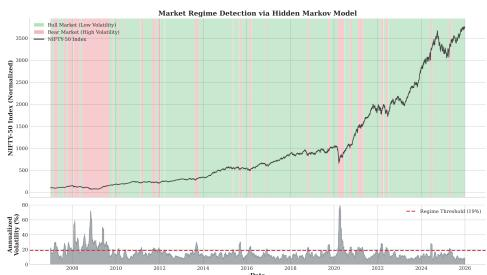
\includegraphics[width=0.74\linewidth]{images/33f0cbdd4e18c1897be25763a9a2422f0e044cbf536822f96ca1ea48c66eb838.jpg}
\figcap{Figure 2. The two-state HMM separates persistent low-volatility expansion (State 0, green) from high-volatility turbulence (State 1, red), capturing the 2020 COVID collapse and the 2022 tightening correction.}
\end{block}

\begin{block}{17 \; Out-of-Sample Wealth Compounding (Fig.~3)}
\centering
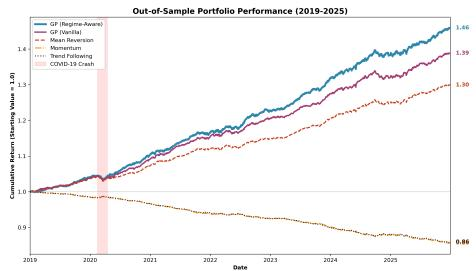
\includegraphics[width=0.74\linewidth]{images/ed7d3491c0ec3faa565111046b72b92898718e516bf5ea024476263ee826a05c.jpg}
\figcap{Figure 3. Cumulative net return, 2019--2025: the regime-aware hybrid compounds through bull and bear phases, while momentum and trend following flatten out ($-40.65\%$ drawdown for momentum).}
\end{block}

\begin{block}{18 \; Rolling Stability \& Discovered Features (Figs.~4,~6)}
\noindent\begin{minipage}[t]{0.45\linewidth}\centering
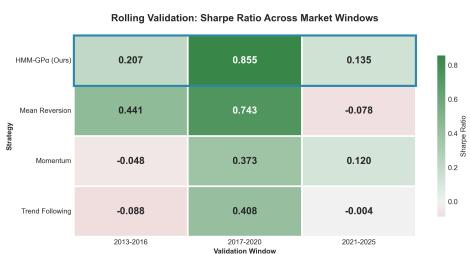
\includegraphics[width=\linewidth]{images/28656a9cc9f26a4ffd2ce0ab7611324d8cd0fff6192ee9abf348a58dd50cc0a7.jpg}
\end{minipage}\hfill
\begin{minipage}[t]{0.45\linewidth}\centering
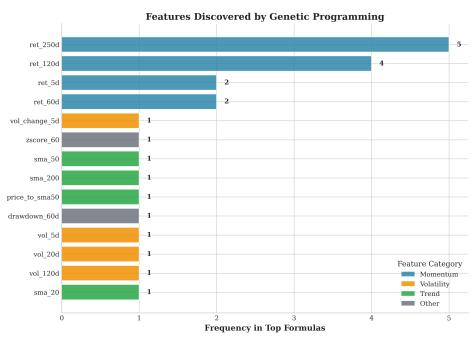
\includegraphics[width=\linewidth]{images/97b82991ea2743e616388671ed37ff6bea3cc310277e70b8b60047cb29f427af.jpg}
\end{minipage}
\figcap{Figure 4 (left). Rolling-window validation Sharpe: HMM-GP$\alpha$ stays positive (0.855) in the turbulent 2017--2020 window where momentum and trend following turn negative. Figure 6 (right). Feature tokens in the top alphas: intermediate momentum and volatility scalers dominate.}
\end{block}

\begin{block}{19 \; Conclusions \& Outlook}
\begin{itemize}
  \item \hl{Sub-period robustness}: positive net Sharpe in \emph{every} macro sub-period (2019 0.72 \textbullet\ 2020 0.58 \textbullet\ 2021 0.76 \textbullet\ 2022 0.51 \textbullet\ 2023--25 0.74); COVID-shock drawdown $-14.82\%$ versus $-38.45\%$ for momentum.
  \item \hl{Economic reading}: the AFM supplies a slow macro anchor while the HMM tracks fast volatility transitions, so evolution finds regime-specific premia instead of averaging contradictory dynamics.
  \item \hl{Capacity \& outlook}: Almgren--Chriss impact implies $\approx$\,\$250M deployable before impact erodes 10\% of net alpha. Next: LoRA-tuned Gemma-2B, multi-agent consensus judging (Llama-3B + Qwen-3B), scaling to NSE 500 / Russell 2000; current limits are reporting lag and a large-cap-only universe.
\end{itemize}
\begin{keybox}{Take-away}
Closed-vocabulary \textbf{semantic repair --- not rejection} is a zero-cost structural regulariser that transfers across Indian, US and Chinese equity panels.
\end{keybox}
\end{block}

\end{column}
\end{columns}

\vskip0.25cm
%================== FOOTER =============================================
\begin{beamercolorbox}[wd=\textwidth,leftskip=0.8cm,rightskip=0.8cm,sep=0.30cm]{cardbox}
{\footnotesize
\textbf{Selected references:} \textbullet\ Kakushadze, \emph{101 Formulaic Alphas}, Wilmott (2016) \textbullet\ Tang, Sun \& Li, \emph{AlphaAgent: automated alpha factor discovery through multimodal LLM agents}, arXiv:2502.16789 (2025) \textbullet\ Chen \& Qi, \emph{TEDE: LLM-assisted semantic pruning for GP alpha mining}, Applied Sciences (2026) \textbullet\ Fortin et al., \emph{DEAP: evolutionary algorithms made easy}, JMLR (2012) \textbullet\ Hamilton, \emph{Econometrica} (1989) \textbullet\ Rabiner, \emph{Proc.\ IEEE} (1989) \textbullet\ McLean \& Pontiff, \emph{J.\ Finance} (2016) \textbullet\ Motghare et al., \emph{FinALFA / multi-document news summarisation}, Computers (2025) \textbullet\ Almgren \& Chriss, \emph{J.\ Risk} (2000).\\[0.1cm]
\textbf{Source:} \code{access.pdf} (IEEE Access manuscript) + MinerU-extracted figure bitmaps in \code{./images} \textbullet\ build with \code{pdflatex poster.tex} (twice).
}
\end{beamercolorbox}

\end{frame}
\end{document}
